\newcommand*{\gennp}{\textbf{TMGenNP}}

\newcommand{\strent}{\rightsquigarrow}
\newcommand{\Rfinal}{R_{\text{final}}}

\newcommand{\bigO}[1]{\mathcal{O}{(#1)}}

\newcommand{\BPR}{\textbf{BinaryPR}}
\newcommand{\fsat}{\textbf{FSAT}}
\newcommand{\sat}{\textbf{SAT}}

\newcommand{\rewwin}[2]{
  \begin{tabular}{C|C|C}
    #1 \\ 
    \midrule #2
  \end{tabular}
}

\newcommand{\blank}{\textbf{\textvisiblespace}}
\newcommand{\delim}{\#}

\newcommand{\polarity}{\textsf{polarity}}


%workaround so that polarities on blanks have the same height as on other symbols
\newcommand*{\TallestContent}{\ensuremath{b}}% <-- This should be the tallest content

\newcommand{\polneg}[1]{\overleftarrow{#1\vphantom{\TallestContent}}}
\newcommand{\polpos}[1]{\overrightarrow{#1\vphantom{\TallestContent}}}
\newcommand{\polneut}[1]{\overline{#1\vphantom{\TallestContent}}}

\newcommand{\reprt}[1]{\ensuremath{\sim_t^{#1}}}
\newcommand{\reprtt}[2]{\ensuremath{\sim_t^{(#1, #2)}}}
\newcommand{\reprc}{\ensuremath{\sim_c}}



\chapter{Informal Overview of the Proof of the Cook-Levin Theorem}\label{chap:informaloverview}
We give an outline of our proof of the Cook-Levin-Threorem, which is loosely based on the presentation by Sipser~\cite{Sipser:TheoryofComputation}. After introducing the problem we reduce from, a tableau construction is presented. We show how we can encode deterministic computations of a Turing machine in such a tableau and later adapt the construction to incorporate a form of nondeterminism. Finally, the structure of the formal proof is described. 

We formally state the main part of the Cook-Levin-Theorem:
\begin{theorem}[Cook-Levin]
  \SAT{} is \NP{}-hard\footnote{From this, we directly get \NP{}-completeness, as was shown by Lemma~\ref{TODO}.}.
\end{theorem}

\section{A Generic Problem for Turing Machines}
Recall that, in order to show a problem $P$ to be \NP{}-hard, we have to show that any problem $Q$ contained in \NP{} can be reduced to it. In our setting of complexity theory in L, we thus have to reduce the computation of L to \SAT{}.
In Section~\ref{TODO}, we argued why it is hard to directly reduce from L to any natural problem. 
Therefore, we believe that the most practical path of reducing from L to \SAT{} is to use Turing machines as an intermediate problem. 

We start from a generic problem for Turing machines. A definition of such a problem the reader might be familiar with is the following:
\begin{center}
  Given a nondeterministic Turing machine $M$, an input $inp$ and a number of steps $t$, does $M$ accept $inp$ in at most $t$ steps?
\end{center}
This definition explicitly employs nondeterminism, making it hard to reason formally. Therefore, we use a characterisation that relates to this one in a similar way the verifier characterisation of \NP{} relates to the one using nondeterminism: the nondeterminism is moved into the input.
\begin{center}
  \gennp{}:
  Given a deterministic Turing machine $M$, a maximal input length $k$ and a number of steps $t$, does there exists an input $inp$ with $\length{inp} \le k$ such that $M$ accepts $inp$ in at most $t$ steps?
\end{center}
Note that we treat the whole input as being a nondeterministic certificate. This does not impose a restriction as the ``regular'' input can just be hardcoded into the Turing machine.


In a theory with Turing machines as the computational model, \gennp{} would be almost trivially \NP{}-hard, although it would not be a natural problem as it depends on the model of computation.
Using L, however, the hardness is not trivial anymore. In this setting, we just see \gennp{} the same as any other problem.\todo{more on that?}

\section{Deterministic Simulation: Tableau of Configurations}
We first consider how the computation of a deterministic Turing machine can be encoded for an arbitrary input of which we only know that its size is at most $k$. The nondetermistic ``guessing'' of an input of such a form will be covered in the next section.

At a first glance, it might seem unintuitive that one can encode the computation of a Turing machine using a fixed-size formula as it is not known a priori how much time or space the Turing machine needs on a particular input.
The key is that \gennp{} just asks us to simulate a Turing machine $M$ for a bounded number of steps $t$ on inputs of a bounded size $\le k$. 
Thus, the formula can be made large enough to account for the worst-case: $t$ computational steps and a space usage of $t + k$ tape cells as the Turing machine can visit at most one cell per computational step\footnote{The bound is $t +k$ and not $t$ since we count the input even if the Turing machine does not read it.}. 

\begin{figure}
  \begin{center}
    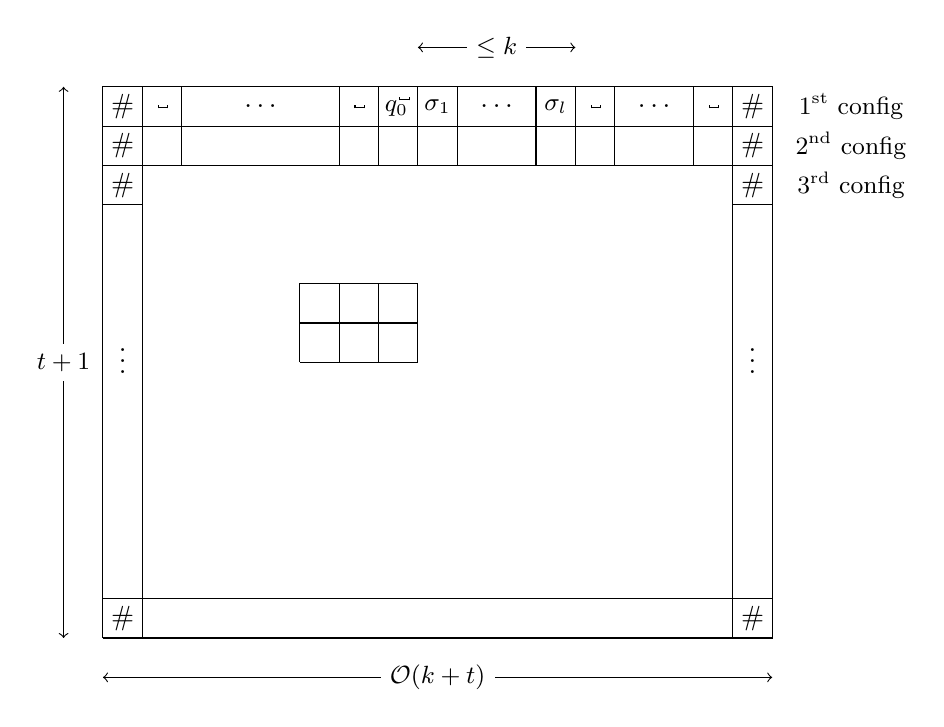
\begin{tikzpicture}
      \draw (1.5, -4) -- (1.5, 3) -- (10, 3) -- (10, -4) -- (1.5, -4);
      \draw (2, -4) -- (2, 3);
      \draw (2.5, 3) -- (2.5, 2);
      \draw (9.5, -4) -- (9.5, 3);
      \draw (1.5, 2.5) -- (10, 2.5);
      \draw (1.5, -3.5) -- (10, -3.5);
      \draw (1.5, 2) -- (10, 2);
      \draw (1.5, 1.5) -- (2, 1.5);
      \draw (9.5, 1.5) -- (10, 1.5);

      \draw (4.5, 3) -- (4.5, 2);
      \draw (5, 3) -- (5, 2);
      \draw (5.5, 3) -- (5.5, 2);
      \draw (6, 3) -- (6, 2);
      \draw (7, 3) -- (7, 2);
      \draw (7.5, 3) -- (7.5, 2);
      \draw (8, 3) -- (8, 2);
      \draw (9, 3) -- (9, 2);
      %\draw (2.5, 3) -- (2.5, 2);
      %\draw (3, 3) -- (3, 2.5);
      %\draw (4.5, 3) -- (4.5, 2.5);
      %\draw (5, 3) -- (5, 2.5);
      %\draw (5.5, 3) -- (5.5, 2.5);
      %\draw (7.5, 3) -- (7.5, 2.5);

      \node at (1.75, 2.75) {\#};
      \node at (1.75, 2.25) {\#};
      \node at (1.75, 1.75) {\#};
      \node at (1.75, -3.75) {\#};
      \node at (9.75, 2.75) {\#};
      \node at (9.75, 2.25) {\#};
      \node at (9.75, 1.75) {\#};
      \node at (9.75, -3.75) {\#};

      \node at (2.25, 2.75) {\textvisiblespace};
      \node at (3.5, 2.75) {$\ldots$};
      \node at (4.75, 2.75) {\textvisiblespace};
      \node at (5.25, 2.75) {\small $q_0^{\blank}$};
      \node at (5.75, 2.75) {\small $\sigma_1$};
      \node at (6.5, 2.75) {$\ldots$};
      \node at (7.25, 2.75) {\small $\sigma_l$};
      \node at (7.75, 2.75) {\textvisiblespace};
      \node at (8.5, 2.75) {$\ldots$};
      \node at (9.25, 2.75) {\textvisiblespace};

      %\node at (6.5, 2.75) {$\ldots$};
      %\node at (5, 2.25) {$\ldots$};

      \node at (1.75, -0.375) {$\vdots$};
      \node at (9.75, -0.375) {$\vdots$};

      \draw (4, -0.5) -- (4, 0.5) -- (5.5, 0.5) -- (5.5, -0.5) -- (4, -0.5);
      \draw (4.5, -0.5) -- (4.5, 0.5);
      \draw (5, -0.5) -- (5, 0.5);
      \draw (4, 0) -- (5.5, 0);

      \path[<->] (1, -4) edge node[fill=white, anchor=center, pos= 0.5] {\small $t+1$} (1, 3);
      \path[<->] (1.5, -4.5) edge node[fill=white, anchor=center, pos=0.5] {\small $\bigO{k + t}$} (10, -4.5);
      \path[<->] (5.5, 3.5) edge node[fill=white, anchor=center, pos=0.5] {\small $\le k$} (7.5, 3.5);

      \node at (11, 2.75) {\small 1\textsuperscript{st} config};
      \node at (11, 2.25) {\small 2\textsuperscript{nd} config};
      \node at (11, 1.75) {\small 3\textsuperscript{rd} config};
    \end{tikzpicture}
  \end{center}
  \caption{The tableau of configurations}\label{fig:tableau}
\end{figure}

With this insight, we write down the computation of the Turing machine in a tableau (Fig.~\ref{fig:tableau}).
The tableau consists of $t+1$ lines, one for each configuration that can be encountered in $t$ computational steps. Each line encodes one configuration consisting of a state symbol and the contents of the tape. We call such a line a \emph{configuration string}. The state symbol is also annotated with the symbol currently under the head.
The first line contains the initial state $q_0$ and the input $\sigma_1, \ldots, \sigma_l$ for $l \le k$, where the head is one symbol to the left of the input (denoted by the blank the state is annotated with).
Note that each line has a fixed length accounting for the maximum number of tape cells the Turing machine can use. However, the Turing machine will usually use less space than is available. The cells unused by a configuration do contain special blanks \blank.
These blanks are not contained in the Turing machine tape alphabet but are part of the tableau encoding, as our Turing machines do not have blanks built-in.
Each line of the tableau is delimited by \delim, the purpose of which will become clear later.
In the end, each cell of the tableau will be represented by a number of Boolean variables used by the \SAT{} formula.

As noted above, the state symbol also contains the current symbol under the head. This choice is clear as it makes the transition taken by the Turing machine only depend on one cell.
However, there are multiple ways of dealing with head movements. 
The most straightforward way might be to move the position of the state symbol, resembling the movement of the head (moving-head semantics).
\begin{example}[Moving Head]\label{ex:movinghead}
  Consider the Turing machine $M$ over alphabet $\Sigma = \{a, b, c\}$ with $Q = \{q_0, q_1\}$, $\textsf{halt}~q_0 = \bfalse$ and $\delta(q_0, \OSome{a}) = (q_1, (\OSome{b}, \movel))$. 
  The successor of the tableau line
  \begin{center}
    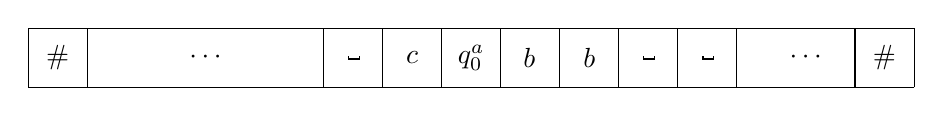
\begin{tikzpicture}
      \draw (-0.75, 0.75) -- (10.5, 0.75);
      \draw (-0.75, 0) -- (10.5, 0);
      \draw (-0.75, 0) -- (-0.75, 0.75);
      \draw (10.5, 0) -- (10.5, 0.75);

      \draw (0, 0) -- (0, 0.75);
      \draw (9.75, 0) -- (9.75, 0.75);
      \node at (-0.375, 0.375) {\#};
      \node at (10.125, 0.375) {\#};

      \draw (4.5, 0) -- (4.5, 0.75);
      \draw (5.25, 0) -- (5.25, 0.75);
      \draw (3.75, 0) -- (3.75, 0.75);
      \draw (3, 0) -- (3, 0.75);
      \draw (6, 0) -- (6, 0.75);
      \draw (6.75, 0) -- (6.75, 0.75);
      \draw (7.5, 0) -- (7.5, 0.75);
      \draw (8.25, 0) -- (8.25, 0.75);

      \node at (1.5, 0.375) {$\cdots$};
      \node at (9.125, 0.375) {$\cdots$};
      \node at (5.6125, 0.375) {$b$};
      \node at (6.375, 0.375) {$b$};
      \node at (7.125, 0.375) {\blank};
      \node at (7.875, 0.375) {\blank};
      \node at (4.875, 0.375) {$q_0^a$};
      \node at (4.125, 0.375) {$c$};
      \node at (3.375, 0.375) {\blank};

    \end{tikzpicture}
  \end{center}
  using moving-head semantics would be 
  \begin{center}
    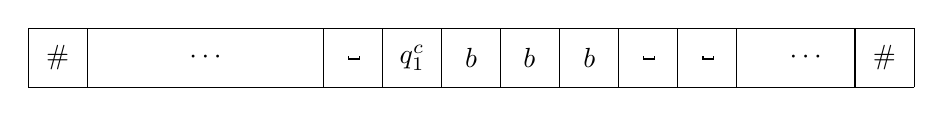
\begin{tikzpicture}
      \draw (-0.75, 0.75) -- (10.5, 0.75);
      \draw (-0.75, 0) -- (10.5, 0);
      \draw (-0.75, 0) -- (-0.75, 0.75);
      \draw (10.5, 0) -- (10.5, 0.75);

      \draw (0, 0) -- (0, 0.75);
      \draw (9.75, 0) -- (9.75, 0.75);
      \node at (-0.375, 0.375) {\#};
      \node at (10.125, 0.375) {\#};

      \draw (4.5, 0) -- (4.5, 0.75);
      \draw (5.25, 0) -- (5.25, 0.75);
      \draw (3.75, 0) -- (3.75, 0.75);
      \draw (3, 0) -- (3, 0.75);
      \draw (6, 0) -- (6, 0.75);
      \draw (6.75, 0) -- (6.75, 0.75);
      \draw (7.5, 0) -- (7.5, 0.75);
      \draw (8.25, 0) -- (8.25, 0.75);

      \node at (1.5, 0.375) {$\cdots$};
      \node at (9.125, 0.375) {$\cdots$};
      \node at (5.6125, 0.375) {$b$};
      \node at (6.375, 0.375) {$b$};
      \node at (7.125, 0.375) {\blank};
      \node at (7.875, 0.375) {\blank};
      \node at (4.875, 0.375) {$b$};
      \node at (4.125, 0.375) {$q_1^c$};
      \node at (3.375, 0.375) {\blank};
    \end{tikzpicture}
  \end{center}
\end{example}

While this behaviour does work, it makes formal reasoning hard: 
Depending on \emph{how} the Turing machine moves its head in order to write down a string, the configuration string will look differently, although it logically represents the same configuration.\todo{make that clearer, maybe with an example?}
Thus, for any given configuration $(q, tp)$ of the machine, there are multiple ways of encoding it as a configuration string:
\begin{center}
  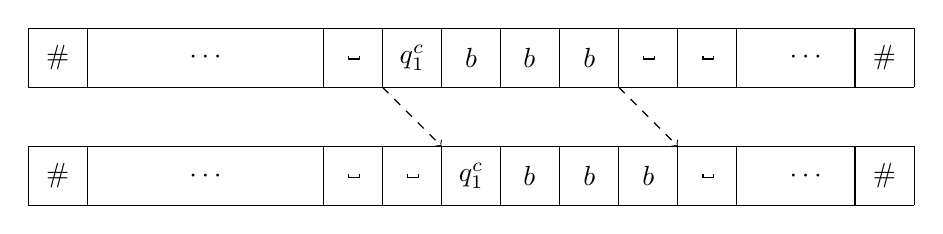
\begin{tikzpicture}
    \draw (-0.75, -0.75) -- (10.5, -0.75);
    \draw (-0.75, 0) -- (10.5, 0);
    \draw (-0.75, 0) -- (-0.75, -0.75);
    \draw (10.5, 0) -- (10.5, -0.75);

    \draw (0, 0) -- (0, -0.75);
    \draw (9.75, 0) -- (9.75, -0.75);
    \node at (-0.375, -0.375) {\#};
    \node at (10.125, -0.375) {\#};

    \draw (4.5, 0) -- (4.5, -0.75);
    \draw (5.25, 0) -- (5.25, -0.75);
    \draw (3.75, 0) -- (3.75, -0.75);
    \draw (3, 0) -- (3, -0.75);
    \draw (6, 0) -- (6, -0.75);
    \draw (6.75, 0) -- (6.75, -0.75);
    \draw (7.5, 0) -- (7.5, -0.75);
    \draw (8.25, 0) -- (8.25, -0.75);

    \node at (1.5, -0.375) {$\cdots$};
    \node at (9.125, -0.375) {$\cdots$};
    \node at (5.6125, -0.375) {$b$};
    \node at (6.375, -0.375) {$b$};
    \node at (7.125, -0.375) {\blank};
    \node at (7.875, -0.375) {\blank};
    \node at (4.875, -0.375) {$b$};
    \node at (4.125, -0.375) {$q_1^c$};
    \node at (3.375, -0.375) {\blank};

    \draw[-{>[scale=2.0]}, dashed] (3.75, -0.75) -- (4.5, -1.5);
    \draw[-{>[scale=2.0]}, dashed] (6.75, -0.75) -- (7.5, -1.5);

    \draw (-0.75, -1.5) -- (10.5, -1.5);
    \draw (-0.75, -2.25) -- (10.5, -2.25);
    \draw (-0.75, -2.25) -- (-0.75, -1.5);
    \draw (10.5, -2.25) -- (10.5, -1.5);

    \draw (0, -2.25) -- (0, -1.5);
    \draw (9.75, -2.25) -- (9.75, -1.5);
    \node at (-0.375, -1.875) {\#};
    \node at (10.125, -1.875) {\#};


    \draw (4.5, -1.5) -- (4.5, -2.25);
    \draw (5.25, -1.5) -- (5.25, -2.25);
    \draw (3.75, -1.5) -- (3.75, -2.25);
    \draw (3, -1.5) -- (3, -2.25);
    \draw (6, -1.5) -- (6, -2.25);
    \draw (6.75, -1.5) -- (6.75, -2.25);
    \draw (7.5, -1.5) -- (7.5, -2.25);
    \draw (8.25, -1.5) -- (8.25, -2.25);

    \node at (1.5, -1.875) {$\cdots$};
    \node at (9.125, -1.875) {$\cdots$};
    \node at (5.6125, -1.875) {$b$};
    \node at (6.375, -1.875) {$b$};
    \node at (7.125, -1.875) {$b$};
    \node at (7.875, -1.875) {\blank};
    \node at (4.875, -1.875) {$q_1^c$};
    \node at (4.125, -1.875) {\blank};
    \node at (3.375, -1.875) {\blank};

  \end{tikzpicture}
\end{center}

Usually one wants to avoid such issues of non-uniqueness.\todo{comment on that in chapter 5 when we do the proofs}
Therefore, we instead use a moving-tape semantics where the position of the head (and thus the state symbol) is fixed at the center of the string. Instead of moving the head, the whole tape is shifted around the head.

\begin{example}[Moving Tape]\label{ex:movingtape}
  Adapting example~\ref{ex:movinghead}, the same transition looks like this when using moving-tape semantics:
  \begin{center}
    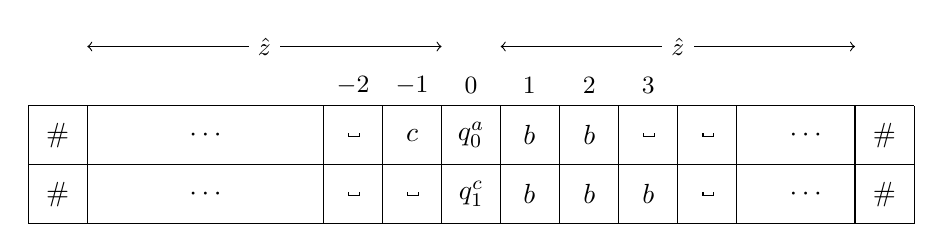
\begin{tikzpicture}
      \draw (-0.75, 0.75) -- (10.5, 0.75);
      \draw (-0.75, 0) -- (10.5, 0);
      \draw (-0.75, 0) -- (-0.75, 0.75);
      \draw (10.5, 0) -- (10.5, 0.75);

      \draw (0, 0) -- (0, 0.75);
      \draw (9.75, 0) -- (9.75, 0.75);
      \node at (-0.375, 0.375) {\#};
      \node at (10.125, 0.375) {\#};

      \draw (4.5, 0) -- (4.5, 0.75);
      \draw (5.25, 0) -- (5.25, 0.75);
      \draw (3.75, 0) -- (3.75, 0.75);
      \draw (3, 0) -- (3, 0.75);
      \draw (6, 0) -- (6, 0.75);
      \draw (6.75, 0) -- (6.75, 0.75);
      \draw (7.5, 0) -- (7.5, 0.75);
      \draw (8.25, 0) -- (8.25, 0.75);

      \node at (5.6125, 1) {\small$1$};
      \node at (6.375, 1) {\small$2$};
      \node at (7.125, 1) {\small$3$};
      \node at (4.875, 1) {\small$0$};
      \node at (4.125, 1) {\small$-1$};
      \node at (3.375, 1) {\small$-2$};

      \node at (1.5, 0.375) {$\cdots$};
      \node at (9.125, 0.375) {$\cdots$};
      \node at (5.6125, 0.375) {$b$};
      \node at (6.375, 0.375) {$b$};
      \node at (7.125, 0.375) {\blank};
      \node at (7.875, 0.375) {\blank};
      \node at (4.875, 0.375) {$q_0^a$};
      \node at (4.125, 0.375) {$c$};
      \node at (3.375, 0.375) {\blank};

      \path[<->] (0, 1.5) edge node[fill=white, anchor=center, pos= 0.5] {\small $\hat{z}$} (4.5, 1.5);
      \node[color=white] at (4.75, 1.5) {l};
      \path[<->] (5.25, 1.5) edge node[fill=white, anchor=center, pos =0.5] {\small $\hat{z}$} (9.75, 1.5);

      \draw (-0.75, -0.75) -- (10.5, -0.75);
      \draw (-0.75, -0.75) -- (-0.75, 0);
      \draw (10.5, -0.75) -- (10.5, 0);

      \draw (0, 0) -- (0, -0.75);
      \draw (9.75, 0) -- (9.75, -0.75);
      \node at (-0.375, -0.375) {\#};
      \node at (10.125, -0.375) {\#};


      \draw (4.5, 0) -- (4.5, -0.75);
      \draw (5.25, 0) -- (5.25, -0.75);
      \draw (3.75, 0) -- (3.75, -0.75);
      \draw (3, 0) -- (3, -0.75);
      \draw (6, 0) -- (6, -0.75);
      \draw (6.75, 0) -- (6.75, -0.75);
      \draw (7.5, 0) -- (7.5, -0.75);
      \draw (8.25, 0) -- (8.25, -0.75);

      \node at (1.5, -0.375) {$\cdots$};
      \node at (9.125, -0.375) {$\cdots$};
      \node at (5.6125, -0.375) {$b$};
      \node at (6.375, -0.375) {$b$};
      \node at (7.125, -0.375) {$b$};
      \node at (7.875, -0.375) {\blank};
      \node at (4.875, -0.375) {$q_1^c$};
      \node at (4.125, -0.375) {\blank};
      \node at (3.375, -0.375) {\blank};
    \end{tikzpicture}
  \end{center}
  Note that the size of the substrings left and right of the center symbol is the same number $\hat{z}$ depending on $t$ and $k$, expressing that the state symbol is fixed at the center.
\end{example}

With the moving-tape representation, we have arrived at a formally pleasing handling of head movements. 

It remains to encode that the successive lines of the tableau follow from each other according to the Turing machine's transition function.
For this, we introduce \emph{rewrite windows} consisting of $3 \times 2$ symbols. 
\begin{center}
  \begin{tabular}{C}
    \arrayrulecolor{white}
    premise\\
    \midrule
    \color{black}conclusion
  \end{tabular}
  \begin{tabular}{C|C|C}
    x_1 & x_2 & x_3 \\ 
    \midrule x_4 & x_5 & x_6
  \end{tabular}
\end{center}

These rewrite windows are used to justify that one line of the tableau \emph{validly} follows from the previous one. At each possible offset, there must exist a rewrite window whose premise matches a prefix of the previous string and whose conclusion matches a prefix of the succeding string.

\begin{example}[Rewrite Windows]\label{ex:rewwindows}
  Consider again example~\ref{ex:movingtape}. For the positions labelled -2, -1, 0, 1 and 2 we need the following rewrite windows (from left to right):
  \begin{center}
    \rewwin{\blank{} & c & q_0^a}{\blank{} & \blank{} & q_1^c}
    \rewwin{c & q_0^a & b}{\blank{} & q_1^c & b}
    \rewwin{q_0^a & b & b}{q_1^c & b & b}
    \rewwin{b & b & \blank}{b & b & b}
    \rewwin{b & \blank{} & \blank{}}{b & b & \blank{}}
  \end{center}
\end{example}

The key behind this construction is that the windows have to overlap. In this way, a global constraint (that the whole configuration string consistently follows from the previous one) is enforced using small local constraints given by the rewrite windows.

We create a set of rewrite windows that encode the valid transitions. 
%In the end, these rewrite windows and the validity constraint are encoded using Boolean formulas. 
Of course, a great number of rewrite windows is needed for that. We mainly have three types of windows: for shifts of the tape, for the transition function involving the center state symbol, and for replicating the final configuration if the Turing machine halts early in less than $t$ steps.

Most of the windows need to exist for every possible combination of tape symbols. For instance, shifting the tape should be possible independently of its contents. Therefore, we introduce \emph{rewrite rules} which are parameterised over variables ranging over, for instance, the tape alphabet.
\begin{example}[Rewrite Rules for Tape Shifts]
  The rewrite window
  \begin{center}
    \rewwin{b & b & \blank{}}{b & b & b}
  \end{center}
  is an instance of the more general rewrite rule
  \begin{center}
    \rewwin{\sigma_1 & \sigma_2 & \blank{}}{\sigma_3 & \sigma_1 & \sigma_2},
  \end{center}
  where $\sigma_i : \Sigma$. 
\end{example}
Note that we distinguish between blanks $\blank$ and elements of $\Sigma$ as $\blank$ is only a part of the representation of configurations as strings.

Seeing this generaliation, one might now realise a problem regarding the tape shifts: the rewrite windows are not provided enough information for the overlapping constraints to enforce a consistent tape shift.
\begin{example}[Inconsistent Tape Shifts]
  We need not only be able to shift the tape to the right, but also leave its position unchanged. For instance, we need the following rewrite rule:
  \begin{center}
    \rewwin{\sigma_1 & \sigma_2 & \blank{}}{\sigma_1 & \sigma_2 & \blank{}}
  \end{center}
  Looking again at Example~\ref{ex:movingtape}, this rule can be applied at the position labelled with 1 to obtain an alternative successor string:
  \begin{center}
    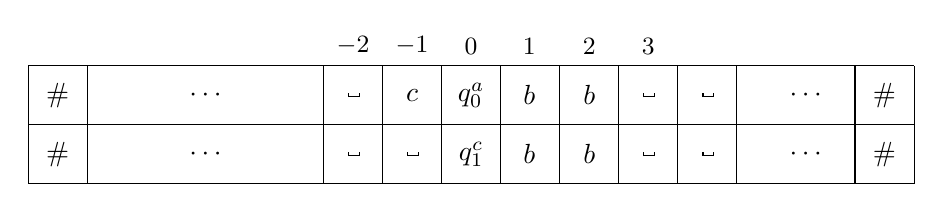
\begin{tikzpicture}
      \draw (-0.75, 0.75) -- (10.5, 0.75);
      \draw (-0.75, 0) -- (10.5, 0);
      \draw (-0.75, 0) -- (-0.75, 0.75);
      \draw (10.5, 0) -- (10.5, 0.75);

      \draw (0, 0) -- (0, 0.75);
      \draw (9.75, 0) -- (9.75, 0.75);
      \node at (-0.375, 0.375) {\#};
      \node at (10.125, 0.375) {\#};

      \draw (4.5, 0) -- (4.5, 0.75);
      \draw (5.25, 0) -- (5.25, 0.75);
      \draw (3.75, 0) -- (3.75, 0.75);
      \draw (3, 0) -- (3, 0.75);
      \draw (6, 0) -- (6, 0.75);
      \draw (6.75, 0) -- (6.75, 0.75);
      \draw (7.5, 0) -- (7.5, 0.75);
      \draw (8.25, 0) -- (8.25, 0.75);

      \node at (5.6125, 1) {\small$1$};
      \node at (6.375, 1) {\small$2$};
      \node at (7.125, 1) {\small$3$};
      \node at (4.875, 1) {\small$0$};
      \node at (4.125, 1) {\small$-1$};
      \node at (3.375, 1) {\small$-2$};

      \node at (1.5, 0.375) {$\cdots$};
      \node at (9.125, 0.375) {$\cdots$};
      \node at (5.6125, 0.375) {$b$};
      \node at (6.375, 0.375) {$b$};
      \node at (7.125, 0.375) {\blank};
      \node at (7.875, 0.375) {\blank};
      \node at (4.875, 0.375) {$q_0^a$};
      \node at (4.125, 0.375) {$c$};
      \node at (3.375, 0.375) {\blank};

      \draw (-0.75, -0.75) -- (10.5, -0.75);
      \draw (-0.75, -0.75) -- (-0.75, 0);
      \draw (10.5, -0.75) -- (10.5, 0);

      \draw (0, 0) -- (0, -0.75);
      \draw (9.75, 0) -- (9.75, -0.75);
      \node at (-0.375, -0.375) {\#};
      \node at (10.125, -0.375) {\#};

      \draw (4.5, 0) -- (4.5, -0.75);
      \draw (5.25, 0) -- (5.25, -0.75);
      \draw (3.75, 0) -- (3.75, -0.75);
      \draw (3, 0) -- (3, -0.75);
      \draw (6, 0) -- (6, -0.75);
      \draw (6.75, 0) -- (6.75, -0.75);
      \draw (7.5, 0) -- (7.5, -0.75);
      \draw (8.25, 0) -- (8.25, -0.75);

      \node at (1.5, -0.375) {$\cdots$};
      \node at (9.125, -0.375) {$\cdots$};
      \node at (5.6125, -0.375) {$b$};
      \node at (6.375, -0.375) {$b$};
      \node at (7.125, -0.375) {$\blank$};
      \node at (7.875, -0.375) {\blank};
      \node at (4.875, -0.375) {$q_1^c$};
      \node at (4.125, -0.375) {\blank};
      \node at (3.375, -0.375) {\blank};
    \end{tikzpicture}
  \end{center}
  This change of configuration is inconsistent: The left half of the tape is shifted to the right, while the right half of the tape is left unchanged.
\end{example}

The reason for this inconsistency is that the rewrite window cannot infer from the overlapping tape symbols alone in which direction the tape is shifted. 
We fix this problem by adding more information: polarities. Polarities $p : \polarity{} \defeq + \bnfmid - \bnfmid \circ{}$ are positive, negative, or neutral. 
Each symbol of the tape alphabet and each blank is annotated with a polarity indicating in which direction the tape is shifted. Polarities do not add any information to the configuration strings in their own right and are just relevant for the configuration changes.
Notationally, we write $\polpos{\sigma}, \polneg{\sigma}, \polneut{\sigma}$ for a symbol $\sigma$ annotated with a positive, negative, or neutral polarity.

\begin{example}[Polarities]\label{ex:polarities}
  The rewrite rules mentioned above now have the following form:
  \begin{center}
    \rewwin{\sigma_1 & \sigma_2 & \blank{}}{\polpos{\sigma_3} & \polpos{\sigma_1} & \polpos{\sigma_2}} 
    \rewwin{\sigma_1 & \sigma_2 & \blank{}}{\polneut{\sigma_1} & \polneut{\sigma_2} & \polneut{\blank{}}}
  \end{center}
  The inconsistent rewrite is not possible anymore as the windows overlapping from the left force a positive polarity.
  \begin{center}
    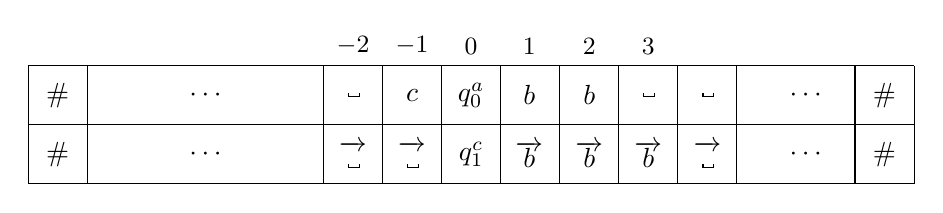
\begin{tikzpicture}
      \draw (-0.75, 0.75) -- (10.5, 0.75);
      \draw (-0.75, 0) -- (10.5, 0);
      \draw (-0.75, 0) -- (-0.75, 0.75);
      \draw (10.5, 0) -- (10.5, 0.75);

      \draw (0, 0) -- (0, 0.75);
      \draw (9.75, 0) -- (9.75, 0.75);
      \node at (-0.375, 0.375) {\#};
      \node at (10.125, 0.375) {\#};

      \draw (4.5, 0) -- (4.5, 0.75);
      \draw (5.25, 0) -- (5.25, 0.75);
      \draw (3.75, 0) -- (3.75, 0.75);
      \draw (3, 0) -- (3, 0.75);
      \draw (6, 0) -- (6, 0.75);
      \draw (6.75, 0) -- (6.75, 0.75);
      \draw (7.5, 0) -- (7.5, 0.75);
      \draw (8.25, 0) -- (8.25, 0.75);

      \node at (5.6125, 1) {\small$1$};
      \node at (6.375, 1) {\small$2$};
      \node at (7.125, 1) {\small$3$};
      \node at (4.875, 1) {\small$0$};
      \node at (4.125, 1) {\small$-1$};
      \node at (3.375, 1) {\small$-2$};

      \node at (1.5, 0.375) {$\cdots$};
      \node at (9.125, 0.375) {$\cdots$};
      \node at (5.6125, 0.375) {$b$};
      \node at (6.375, 0.375) {$b$};
      \node at (7.125, 0.375) {\blank};
      \node at (7.875, 0.375) {\blank};
      \node at (4.875, 0.375) {$q_0^a$};
      \node at (4.125, 0.375) {$c$};
      \node at (3.375, 0.375) {\blank};

      \draw (-0.75, -0.75) -- (10.5, -0.75);
      \draw (-0.75, -0.75) -- (-0.75, 0);
      \draw (10.5, -0.75) -- (10.5, 0);

      \draw (0, 0) -- (0, -0.75);
      \draw (9.75, 0) -- (9.75, -0.75);
      \node at (-0.375, -0.375) {\#};
      \node at (10.125, -0.375) {\#};

      \draw (4.5, 0) -- (4.5, -0.75);
      \draw (5.25, 0) -- (5.25, -0.75);
      \draw (3.75, 0) -- (3.75, -0.75);
      \draw (3, 0) -- (3, -0.75);
      \draw (6, 0) -- (6, -0.75);
      \draw (6.75, 0) -- (6.75, -0.75);
      \draw (7.5, 0) -- (7.5, -0.75);
      \draw (8.25, 0) -- (8.25, -0.75);

      \node at (1.5, -0.375) {$\cdots$};
      \node at (9.125, -0.375) {$\cdots$};
      \node at (5.6125, -0.375) {$\polpos{b}$};
      \node at (6.375, -0.375) {$\polpos{b}$};
      \node at (7.125, -0.375) {$\polpos{b}$};
      \node at (7.875, -0.375) {$\polpos{\blank}$};
      \node at (4.875, -0.375) {$q_1^c$};
      \node at (4.125, -0.375) {$\polpos{\blank}$};
      \node at (3.375, -0.375) {$\polpos{\blank}$};
    \end{tikzpicture}
  \end{center}
\end{example}

Note that we omit the polarities in the premises of rules as they are irrelevant.
Formally, for each of the rewrite rules depicted in Example~\ref{ex:polarities}, we do an instantiation not only for all possible combinations of variable valuations, but also for the three possible polarities in the premise (we only require that the polarities are consistent).

\begin{remark}[Blanks and Polarities]
  Formally, it is not necessary for blanks to be annotated with polarities. However, adding polarities to blanks allows us to handle symbols of the tape alphabet and blanks in a more uniform way, simplifying the formal proofs. 
\end{remark}

Finally, we need to enforce that the final configuration is a halting configuration. This can be encoded by requiring that an element of $[q^m~|~\textsf{halt}~q = \btrue, m : \Sigma + \{\blank\}]$ is contained in the last line of the tableau.\todo{fix notation for type}

\section{Nondeterministic Input}\label{sec:informal_nondet}
The construction presented in the previous section can simulate a deterministic Turing machine given an initial configuration. \gennp{}, however, asks for the existence of an input which the Turing machine accepts. 
This nondeterminism of the input can be encoded by prepending a new line to the tableau:
\begin{center}
  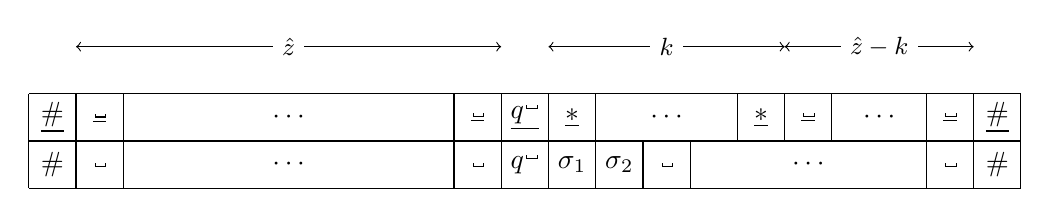
\begin{tikzpicture}[scale=1.2]
    \draw (0, 0.5) -- (10.5, 0.5);
    \draw[thick] (0, 0) -- (10.5, 0);
    \draw (0, 0) -- (0, 0.5);
    \draw (10.5, 0) -- (10.5, 0.5);

    \draw (0.5, 0.5) -- (0.5, 0);
    \draw (1, 0.5) -- (1, 0);
    \draw (10, 0.5) -- (10, 0);
    \draw (9.5, 0.5) -- (9.5, 0);
    \draw (5, 0.5) -- (5, 0);
    \draw (5.5, 0.5) -- (5.5, 0);
    \draw (4.5, 0.5) -- (4.5, 0);
    \draw (6, 0.5) -- (6, 0);
    \draw (7.5, 0.5) -- (7.5, 0);
    \draw (8, 0.5) -- (8, 0);
    \draw (8.5, 0.5) -- (8.5, 0);

    \node at (9, 0.25) {$\cdots$};
    \node at (6.75, 0.25) {$\cdots$};
    \node at (2.75, 0.25) {$\cdots$};

    \node at (0.25, 0.25) {\underline{\#}};
    \node at (0.75, 0.24) {$\underline{\blank}$};
    \node at (4.75, 0.25) {$\underline{\blank}$};
    \node at (5.25, 0.25) {$\underline{q^{\blank}}$};
    \node at (5.75, 0.25) {$\underline{*}$};
    \node at (7.75, 0.25) {$\underline{*}$};
    \node at (8.25, 0.25) {$\underline{\blank}$};
    \node at (9.75, 0.25) {$\underline{\blank}$};
    \node at (10.25, 0.25) {\underline{\#}};

    \draw (0, -0.5) -- (10.5, -0.5);
    \draw (0, 0) -- (0, -0.5);
    \draw (10.5, 0) -- (10.5, -0.5);

    \draw (0.5, -0.5) -- (0.5, 0);
    \draw (1, -0.5) -- (1, 0);
    \draw (10, -0.5) -- (10, 0);
    \draw (9.5, -0.5) -- (9.5, 0);
    \draw (5, -0.5) -- (5, 0);
    \draw (5.5, -0.5) -- (5.5, 0);
    \draw (4.5, -0.5) -- (4.5, 0);
    \draw (6, -0.5) -- (6, 0);
    \draw (6.5, -0.5) -- (6.5, 0);
    \draw (7, -0.5) -- (7, 0);
    %\draw (7.5, -0.5) -- (7.5, 0);
    %\draw (8, -0.5) -- (8, 0);
    %\draw (8.5, -0.5) -- (8.5, 0);

    \node at (2.75, -0.25) {$\cdots$};
    \node at (0.25, -0.25) {\#};
    \node at (0.75, -0.25) {\blank};
    \node at (4.75, -0.25) {\blank};
    \node at (5.25, -0.25) {$q^{\blank}$};
    \node at (5.75, -0.25) {$\sigma_1$};
    \node at (6.25, -0.25) {$\sigma_2$};
    \node at (6.75, -0.25) {\blank};
    \node at (8.25, -0.25) {$\cdots$};
    \node at (9.75, -0.25) {\blank};
    \node at (10.25, -0.25) {\#};

    \path[<->] (5.5, 1) edge node[fill=white, anchor=center, pos= 0.5] {\small $k$} (8, 1);
    \path[<->] (0.5, 1) edge node [fill = white, anchor=center, pos=0.5] {\small $\hat{z}$} (5, 1);
    \path[<->] (8, 1) edge node [fill = white, anchor =center, pos=0.5] {\small $\hat{z}-k$} (10, 1);
  \end{tikzpicture}
\end{center}

The idea is to add rewrite rules which can replace the $\underline{*}$ (wildcard) symbols by arbitrary elements of the tape alphabet. If one wildcard is replaced by a blank, all the other wildcards right of it also need to be replaced by blanks in order to ensure that the used tape region is contiguous. 

\section{Intermediate Problems}
In the presentation by Sipser~\cite{Sipser:TheoryofComputation}, the tableau is directly encoded as a CNF. Doing this formally seems to be hard as one needs to handle the invariants of simulating the Turing machine, the representation of symbols of an arbitrary finite alphabet and the encoding as a CNF all at once. 
Instead, we factorise the proof into smaller parts by introducing three intermediate problems that deal with these concerns one-by-one. 
Figure~\ref{fig:redoverview} gives an overview over the reductions.

The reduction of \gennp{} to Parallel Rewriting (\PR{}), a string-based problem which will be introduced in Section~\ref{sec:pr}, handles the main part of the Turing machine simulation. After that, we do not have to reason about Turing machines anymore. 
Parallel Rewriting can be seen as a model between Turing machines and circuits.
%The remaining three reductions subsequently deal with the encoding of the alphabet, the encoding as a Boolean formula and the conversion to a CNF.

\begin{figure}
  \begin{center}
    \begin{tikzpicture}[scale=0.9, every node/.style={scale=0.9}]
      \node[rectangle, draw=black, minimum width=13cm] (gennp) {Generic Problem on Turing Machines (\gennp{})}; 
      \node[rectangle, draw=black, minimum width = 13cm, below = of gennp] (strrew1) {Parallel Rewriting (\PR{}) on arbitrary $\Sigma$};
      \node[rectangle, draw=black, below = of strrew1, minimum width = 13cm] (strrew2) {Binary Parallel Rewriting};
      \node[rectangle, draw=black, below = of strrew2, minimum width = 13cm] (csat) {Propositional SAT (\fsat{})};
      \node[rectangle, draw=black, below = of csat, minimum width = 13cm] (sat) {SAT on CNFs (\sat{})};
      \draw[->] 
        (gennp) edge node[right] {tableau construction} (strrew1)
        (strrew1) edge node[right] {string homomorphism} (strrew2)
        (strrew2) edge node[right] {encode bits using Boolean variables} (csat)
        (csat) edge node[right] {Tseytin transformation} (sat);
    \end{tikzpicture}
  \end{center}
  \caption{The chain of reductions from \gennp{} to \SAT{}.}\label{fig:redoverview}
\end{figure}


